

\todo{add a figure here showing the total delayed neutron yield}
The equation for which is given by \cite{huynh2014calculation}. This shows the delayed neutrons per fission event.
\begin{figure}[!ht]
    \centering
    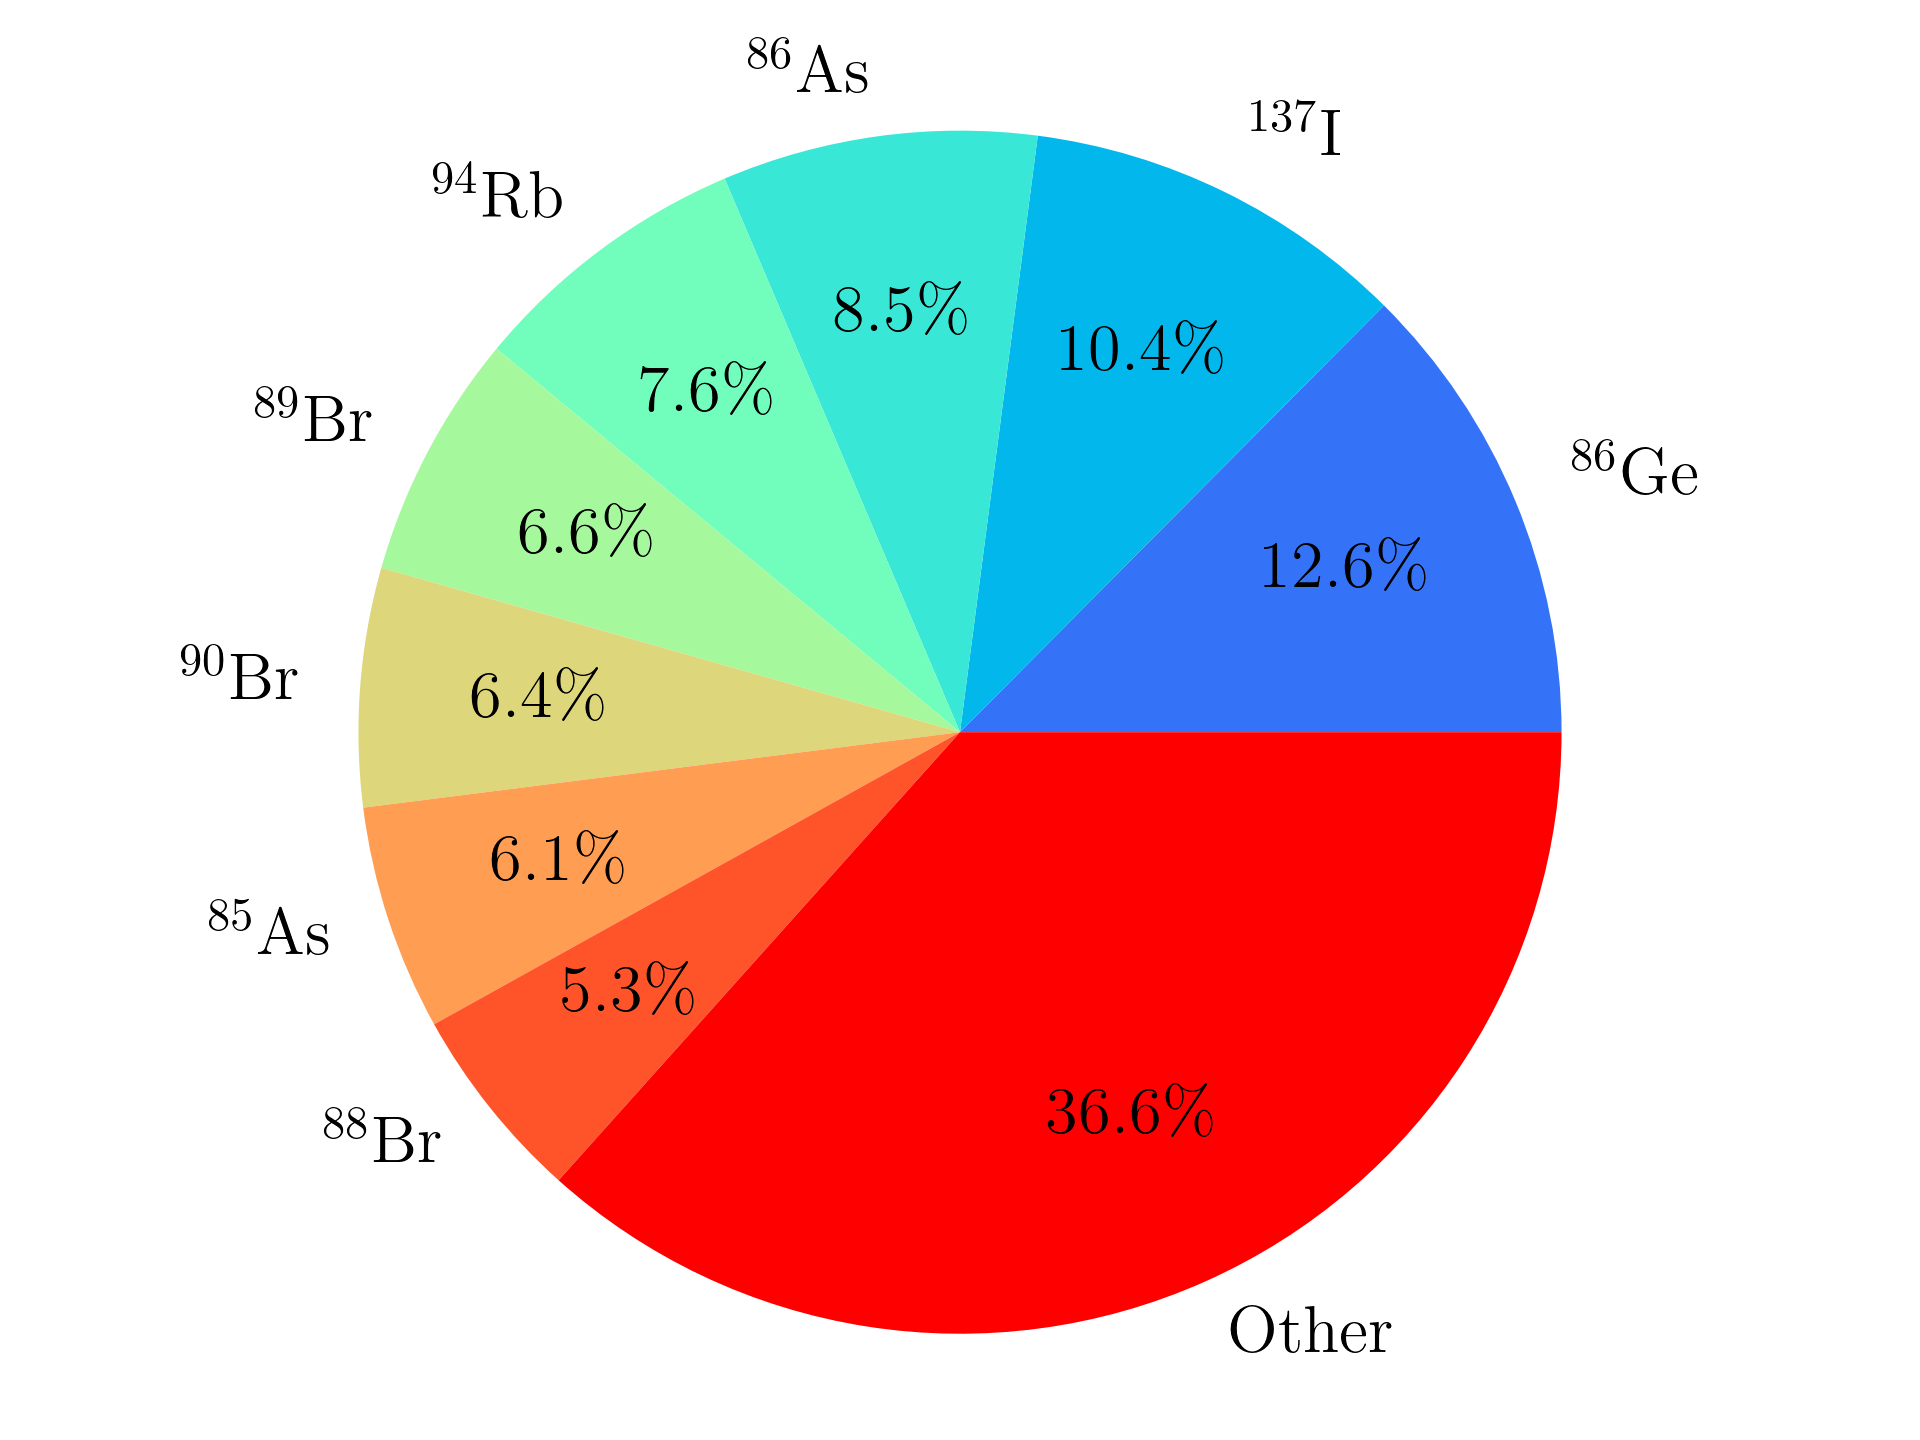
\includegraphics[width=0.5\linewidth]{images/dnp_yield.png}
    \caption{Caption}
    \label{fig:placeholder}
\end{figure}

An alternative which may be interesting is the yield of neutrons from the total irradiation rather than per fission.
To calculate this, simply integrate the delayed neutron counts (Pn*N).

The equation for which is given by \cite{huynh2014calculation}. This shows the delayed neutrons per fission event.
\begin{figure}[!ht]
    \centering
    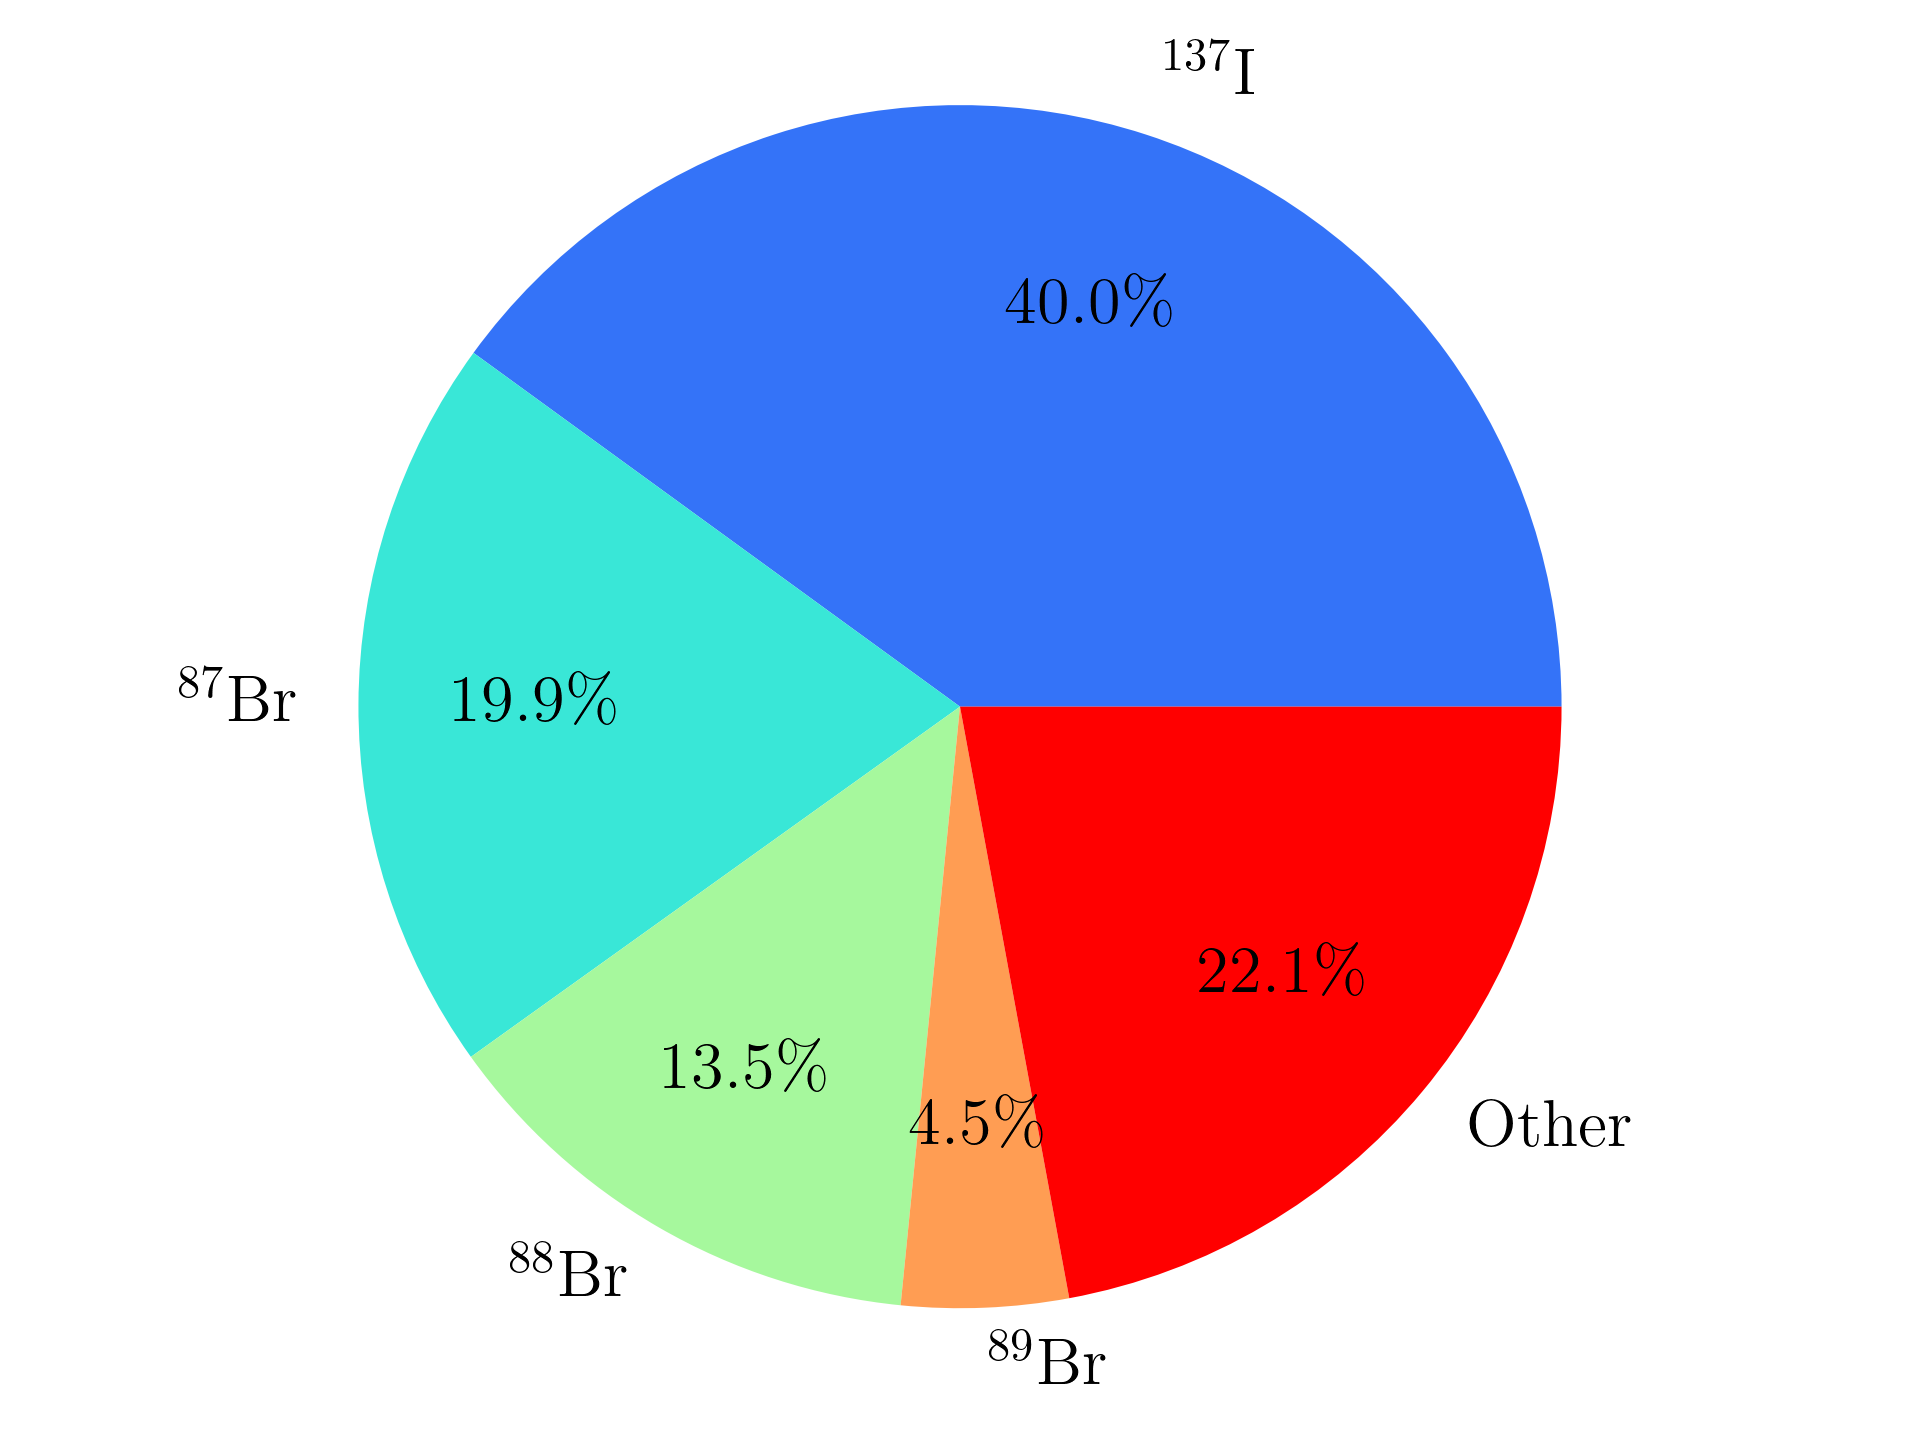
\includegraphics[width=0.5\linewidth]{images/dnp_yield_full_irrad.png}
    \caption{Caption}
    \label{fig:placeholder}
\end{figure}

Top 2 at each time step.
\begin{figure}[!ht]
    \centering
    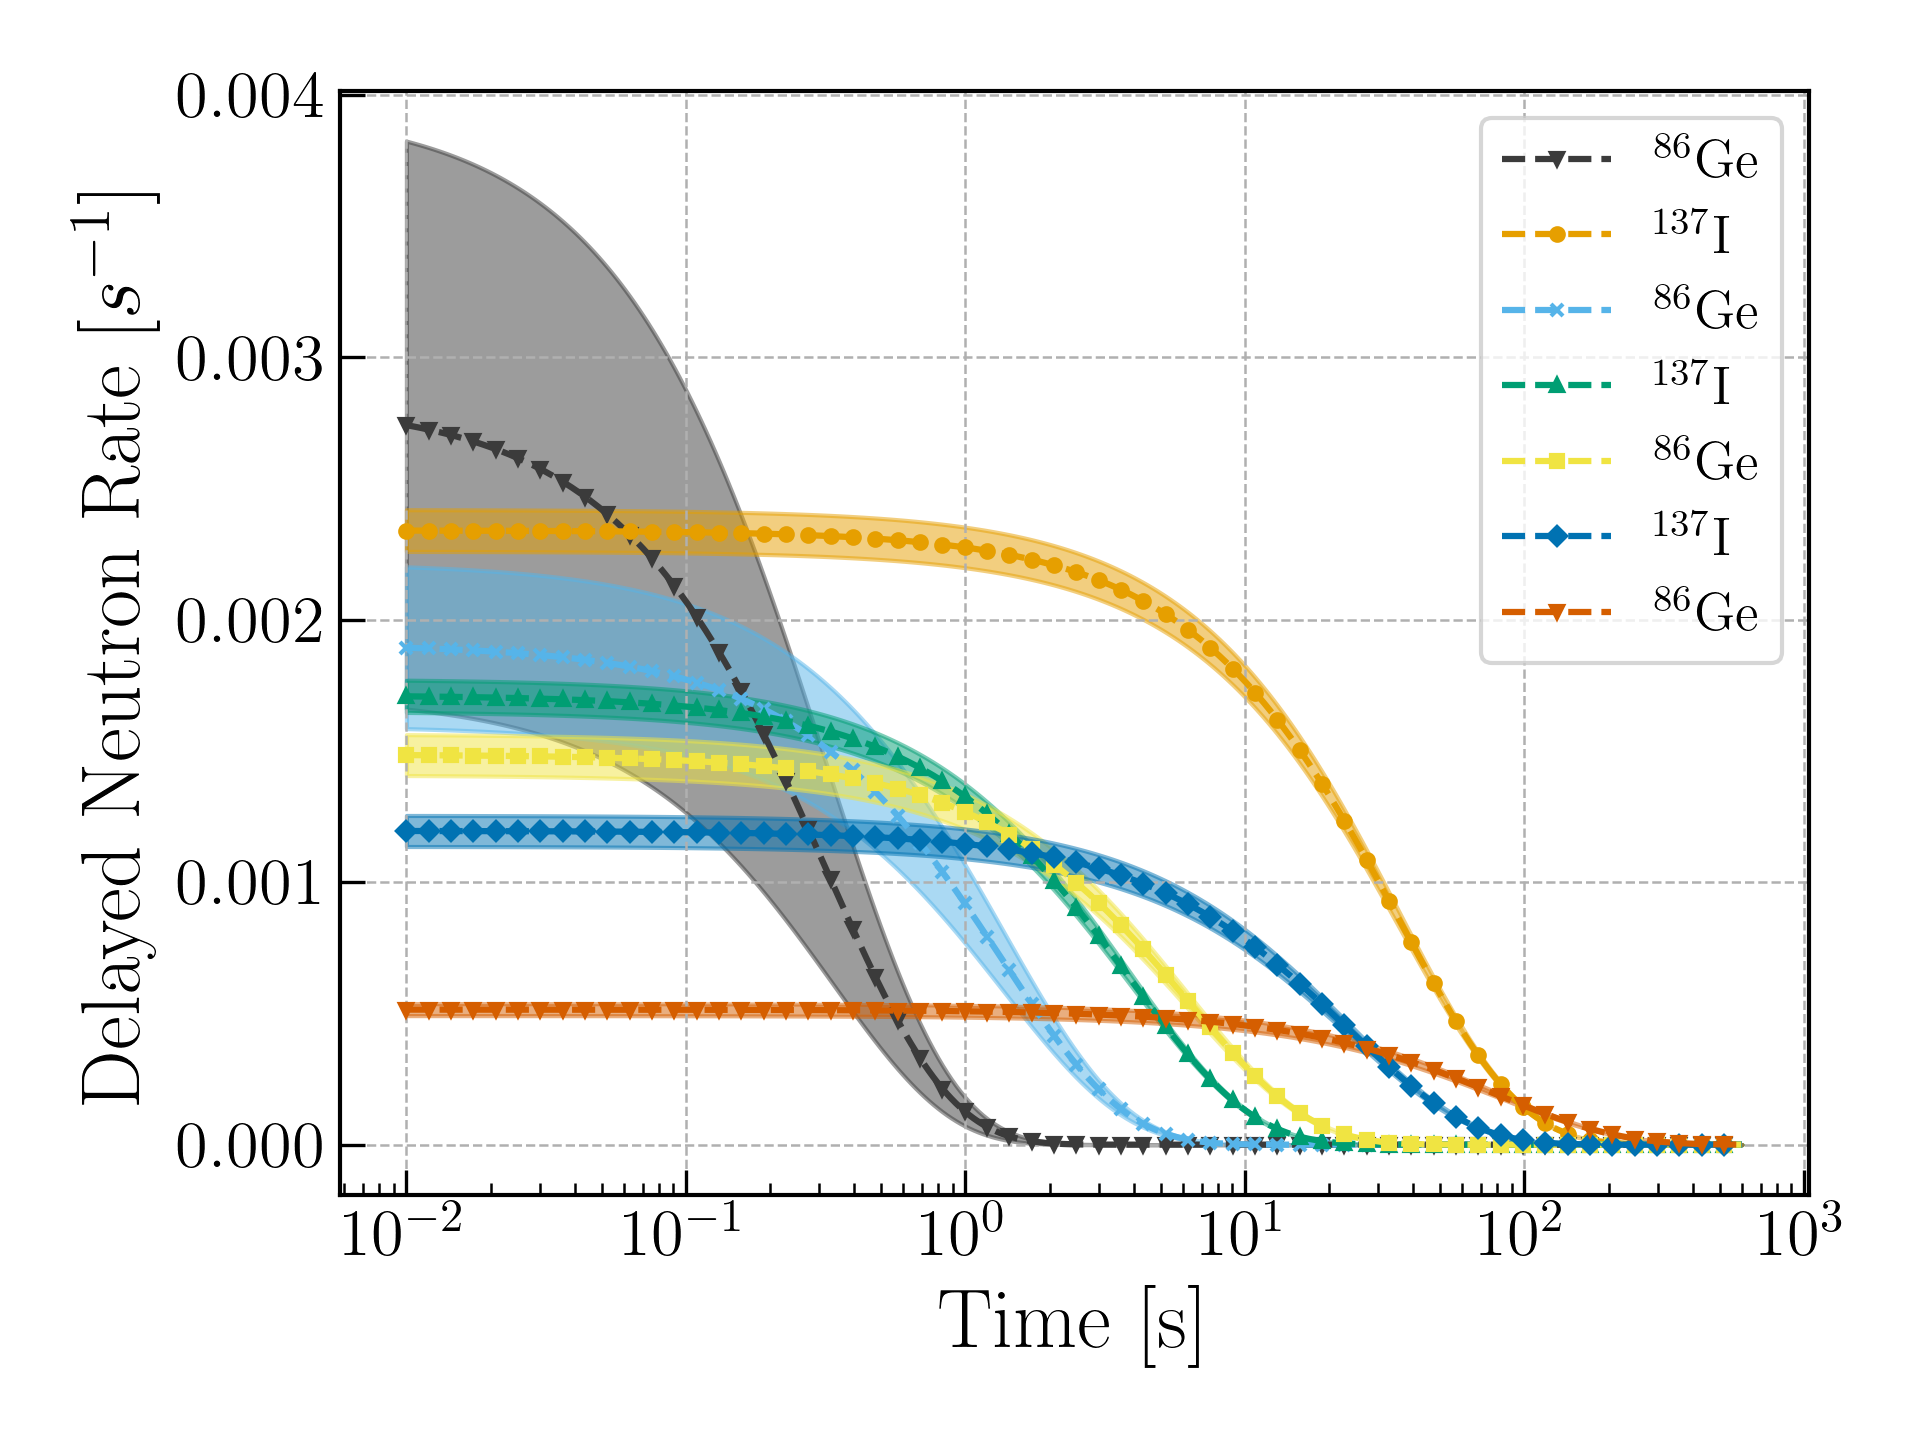
\includegraphics[width=0.5\linewidth]{images/individual_nuclide_rates.png}
    \caption{Caption}
    \label{fig:placeholder}
\end{figure}

\begin{figure}[!ht]
    \centering
    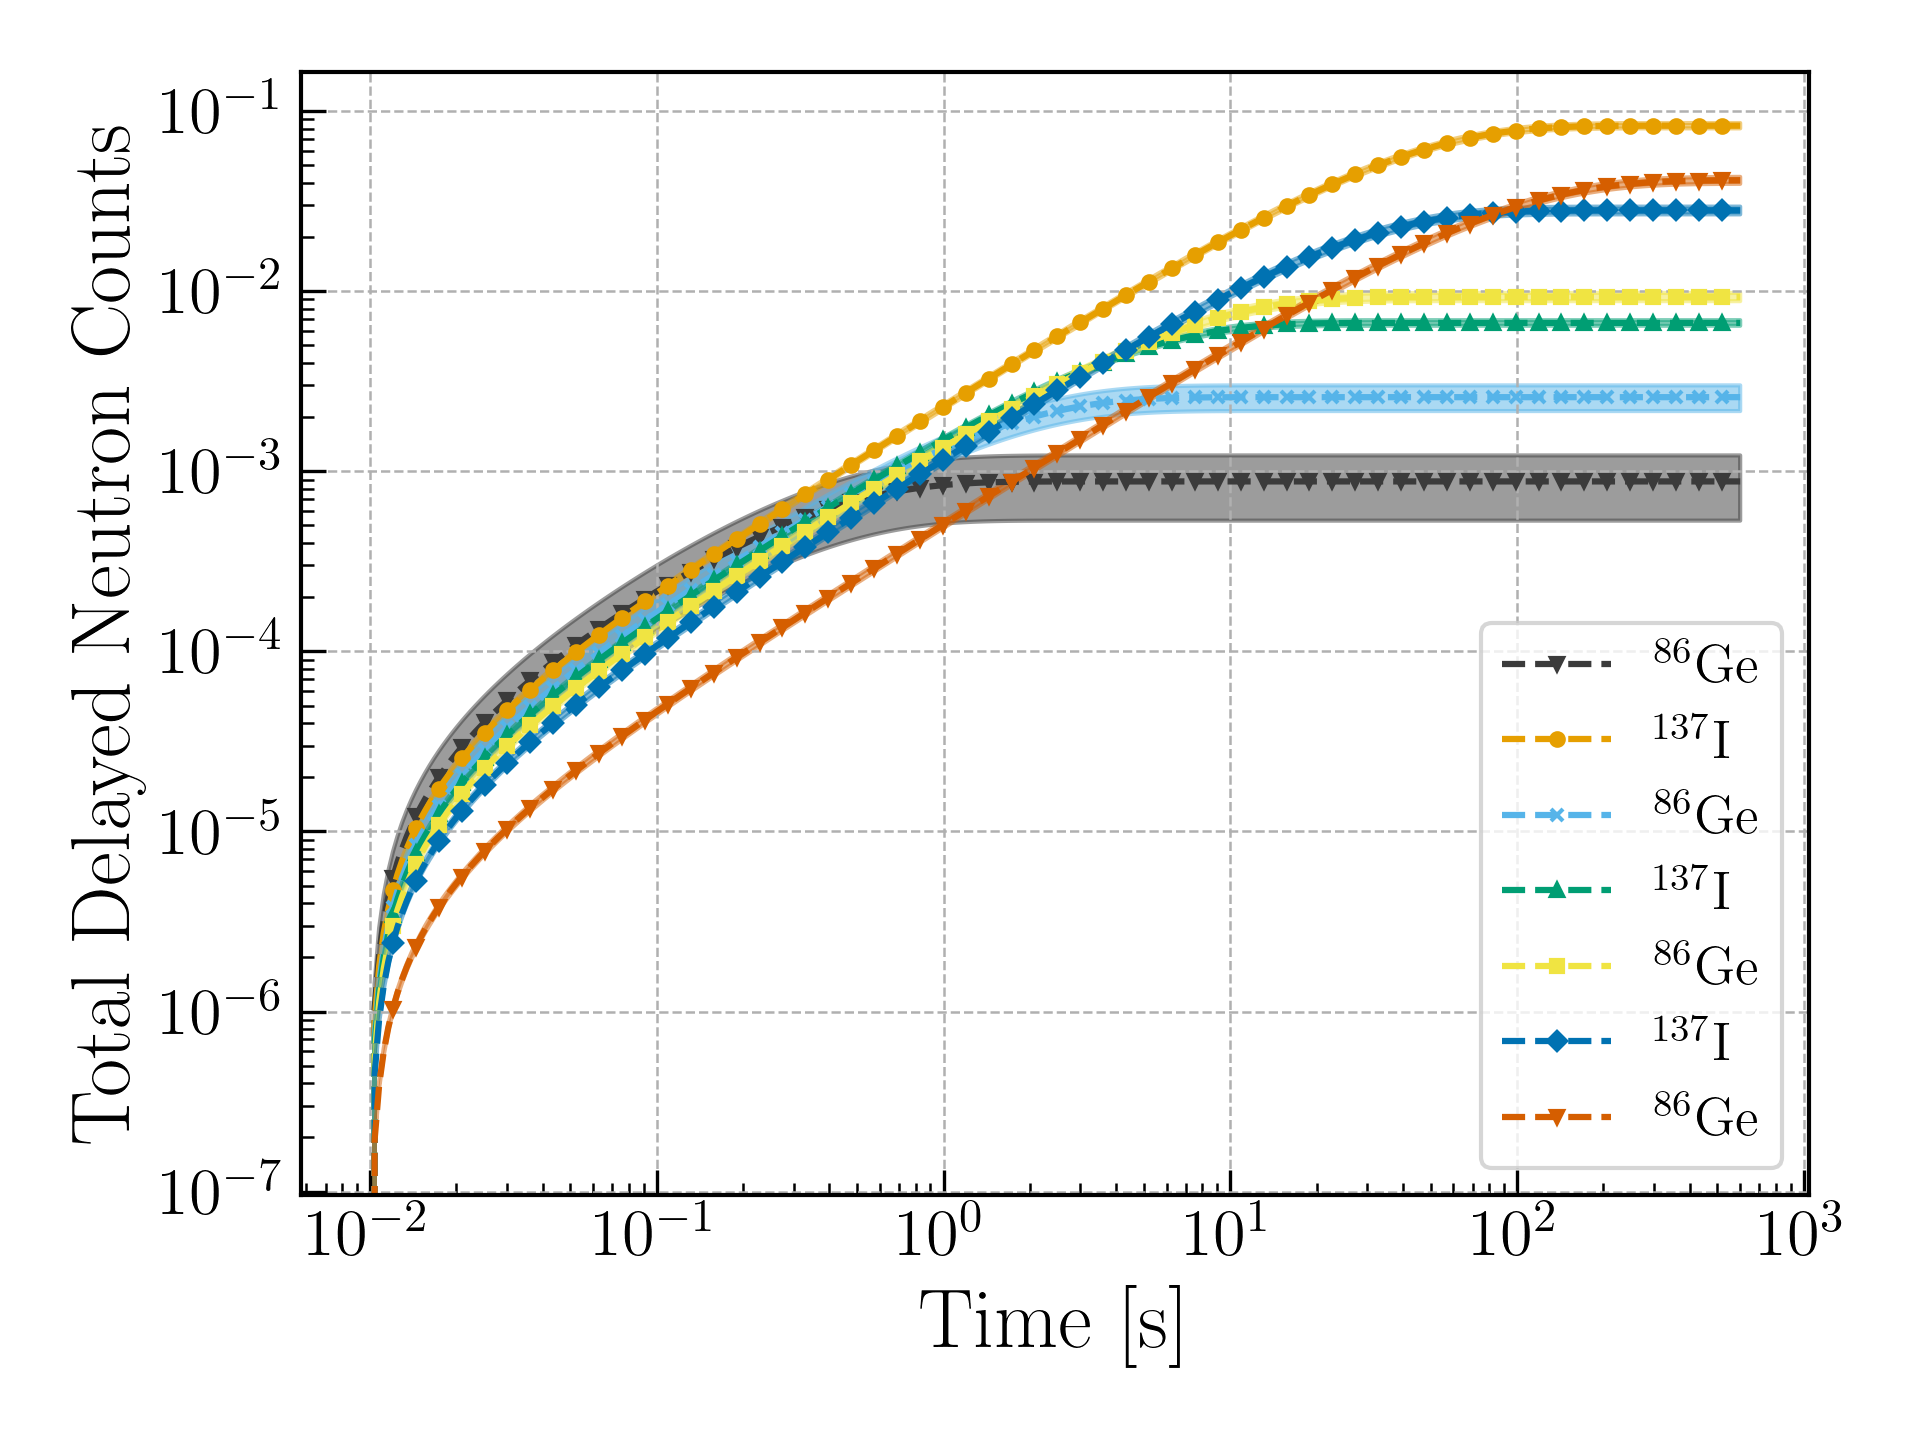
\includegraphics[width=0.5\linewidth]{images/individual_nuclide_counts.png}
    \caption{Caption}
    \label{fig:placeholder}
\end{figure}

\begin{figure}[!ht]
    \centering
    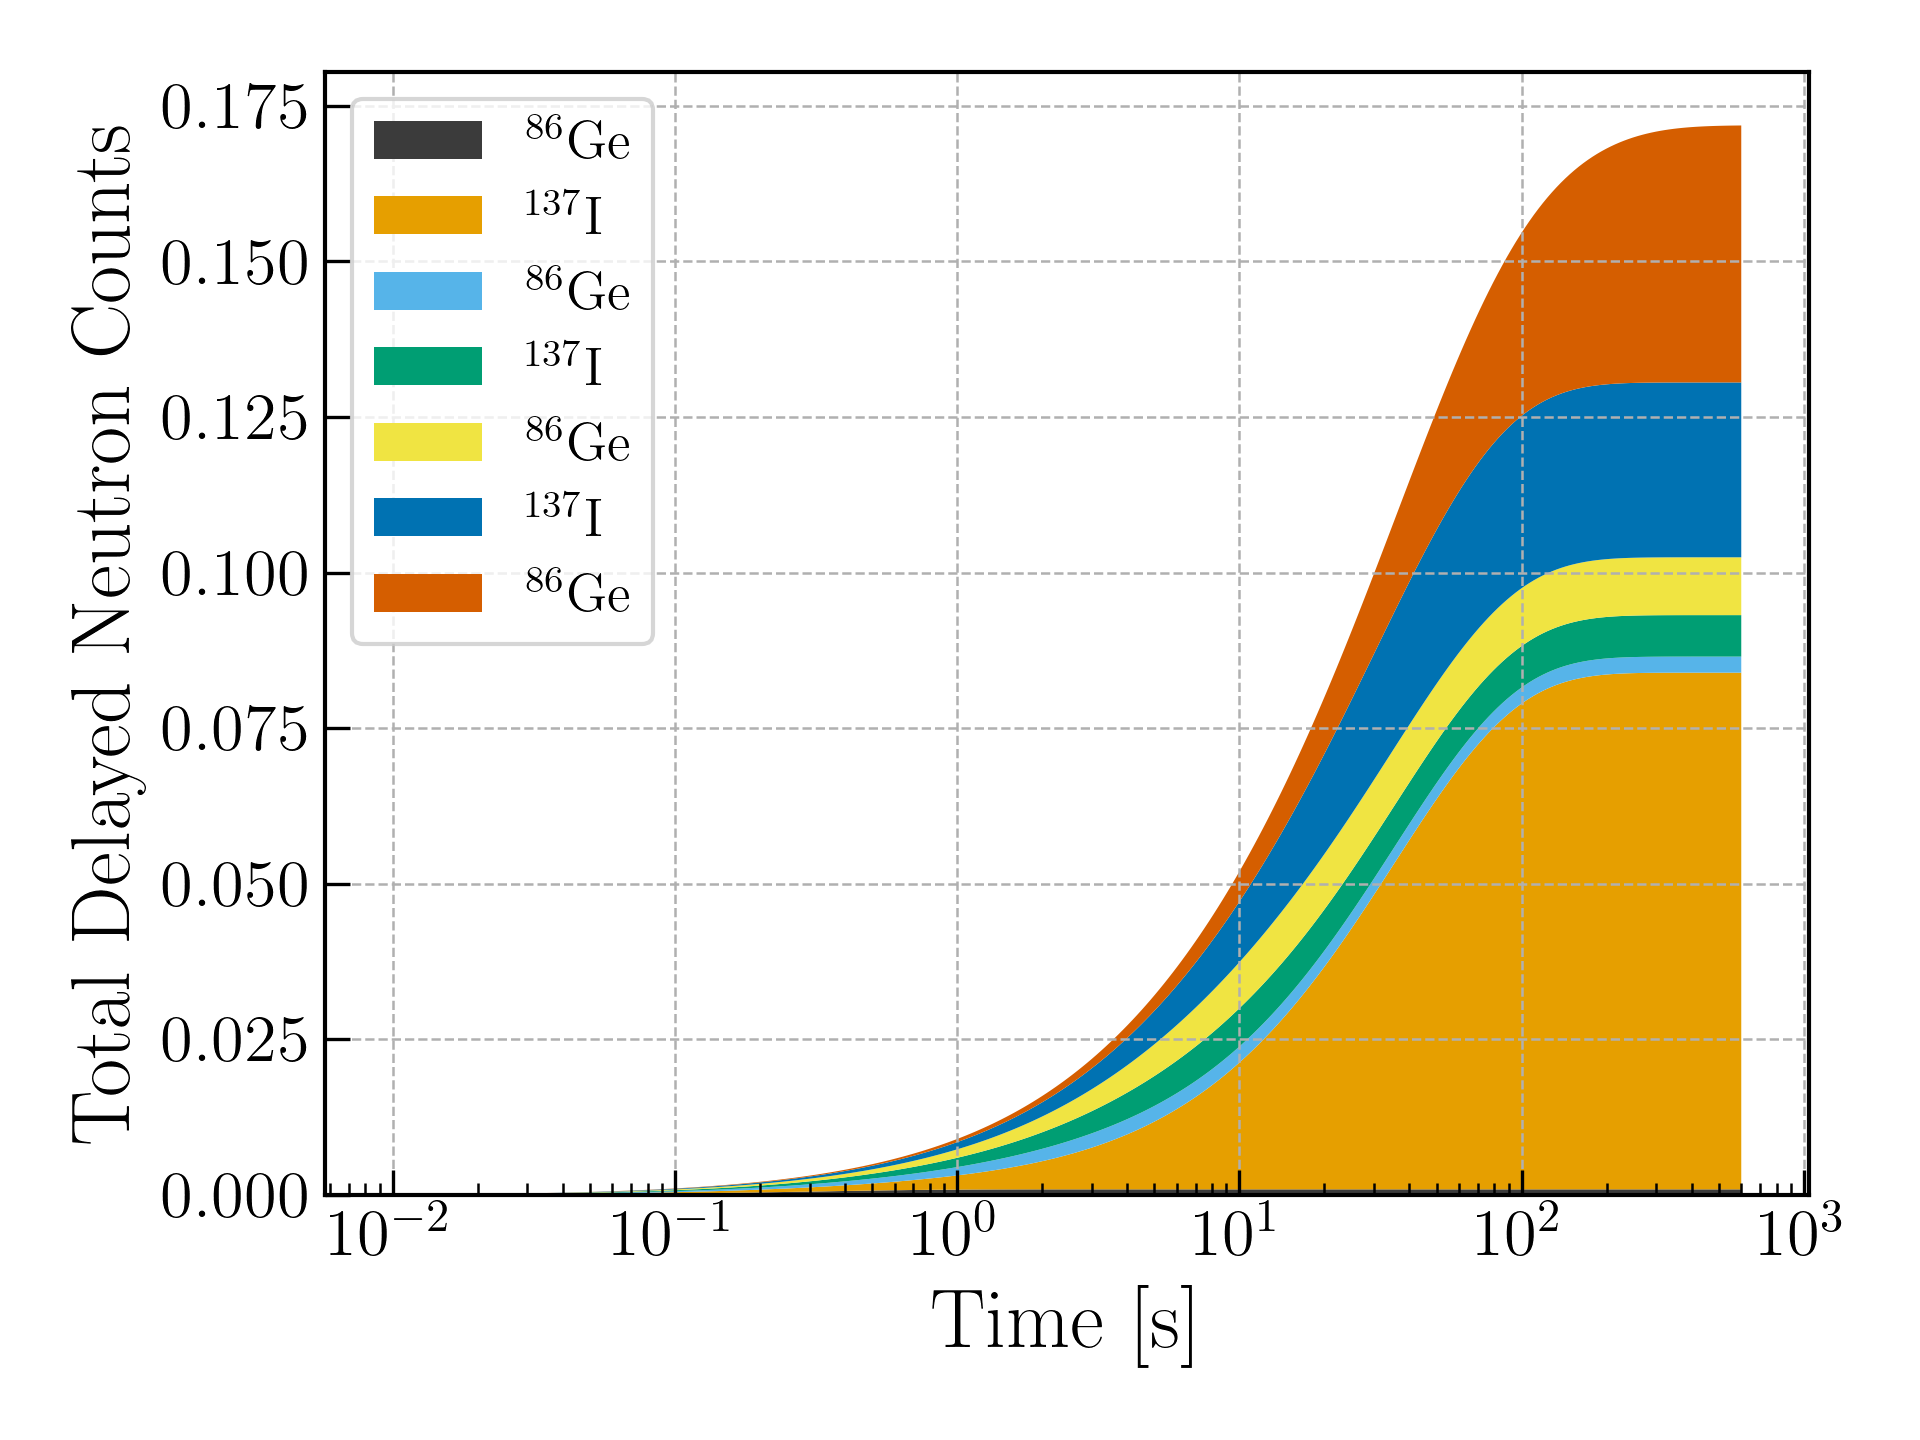
\includegraphics[width=0.5\linewidth]{images/individual_nuclide_counts_stacked.png}
    \caption{Caption}
    \label{fig:placeholder}
\end{figure}

The summed avg halflife doesn't use the non-standard avg halflife equation \cite{parish1999status}.
When it does, 9.2 seconds. When it doesn't, 6.4 seconds.

Summed Vals
0.02254145659046882 $\pm$ 0.0015166459277329472
6.385209000563604 $\pm$ 0.38007097622923025
Group Vals
0.02239 $\pm$ 0.00126
6.40289 $\pm$ 0.33653


summed yield=0.02254145659046882+/-0.0015166459277329472 group yield=0.02239+/-0.00126
summed avg halflife=9.211909360152688+/-0.5483265125917376 group avg halflife=9.23741+/-0.48551
